\documentclass[a4paper]{article}
\usepackage{graphicx}
\usepackage{amssymb}
\usepackage{fancyhdr}
\usepackage{hyperref}
\usepackage{lastpage}
\usepackage[dvipsnames]{xcolor}
\pagestyle{fancy}
\rhead{Andrea Vicari}
\lhead{Smart-IVC: Enhanced Visualization of Cities, \\Through Smart Visual Queries}
\fancyfoot[C]{Page\ \thepage\ of\ \pageref{LastPage}}
\renewcommand{\headrulewidth}{0.4pt}
\renewcommand{\footrulewidth}{0.4pt}

\begin{document}

\begin{titlepage}

\newcommand{\HRule}{\rule{\linewidth}{0.5mm}} % Defines a new command for the horizontal lines, change thickness here

\center % Center everything on the page
 
%----------------------------------------------------------------------------------------
%	HEADING SECTIONS
%----------------------------------------------------------------------------------------
\textsc{\LARGE Universit\'a della Svizzera italiana}\\[1.5cm] % Name of your university/college
\textsc{\Large Faculty of Informatics}\\[0.5cm] % Major heading such as course name
\textsc{\large Bachelor Project Plan\\Spring Semester 2017}\\[0.5cm] % Minor heading such as course title

%----------------------------------------------------------------------------------------
%	TITLE SECTION
%----------------------------------------------------------------------------------------

\HRule \\[0.4cm]
{ \Huge \bfseries Smart-IVC}\\[0.4cm] % Title of your document
{ \huge Enhanced Visualization of Cities, Through Smart Visual Queries}
\HRule \\[1.5cm]
 
%----------------------------------------------------------------------------------------
%	AUTHOR SECTION
%----------------------------------------------------------------------------------------

\begin{minipage}{0.4\textwidth}
\begin{flushleft} \large
\emph{Author:}\\
Andrea \textsc{Vicari} % Your name
vicara@usi.ch % Your name
\end{flushleft}
\end{minipage}
~
\begin{minipage}{0.4\textwidth}
\begin{flushright} \large
\emph{Advisor:} \\
Prof. Michele \textsc{Lanza} % Supervisor's Name
\emph{Assistant:} \\
Dr. Andrea \textsc{Mocci} % Supervisor's Name
\end{flushright}
\end{minipage}\\[4cm]

%----------------------------------------------------------------------------------------
%	DATE SECTION
%----------------------------------------------------------------------------------------

{\large \today}\\[3cm] % Date, change the \today to a set date if you want to be precise

%----------------------------------------------------------------------------------------
%	LOGO SECTION
%----------------------------------------------------------------------------------------


 
%----------------------------------------------------------------------------------------

\vfill % Fill the rest of the page with whitespace

\end{titlepage}
\section*{1. Plan}
\subsection*{Tasks and Milestones}
The tasks that will lead to the final result of this Bachelor Project are going to be the following:
\begin{itemize}
	\item {\bf Study Technologies} (1 week): choose the most suitable technologies for the project
	\item {\bf Build Back End} (2 weeks): retrieve data, model it, store the result in the database and create the APIs.
	\item {\bf Build Front-End GUI} (1 week): that consists in creating the basic skeleton of the website (i.e. menu and buttons) and it work with the APIs
\end{itemize}
Here I put the {\bf first milestone} (M1), therefore, by the end of March the Server and the basic GUI has to be ready.
\begin{itemize}
	\item {\bf Create 3D-Map} (4 weeks): create a 2.5D map and then add height to buildings and details to the map
	\item {\bf Create Interactions in 3D-Map} (3 weeks): make the entities on the map interactive clicking on them
\end{itemize}
Here I put the {\bf second milestone} (M2), therefore, by the first decade of May there must be a working 3D model of the city where is possible to execute queries on the entities
\begin{itemize}
	\item {\bf Test and Finish Work} (2 weeks): complete undone work, test the application and make the necessary fixes
	\item {\bf Write Thesis} (8 weeks): that includes writing the project report, the poster and the final plan
\end{itemize}
Here I present the graphical timeline of the tasks and milestones I described above:\\

\hspace*{-1cm}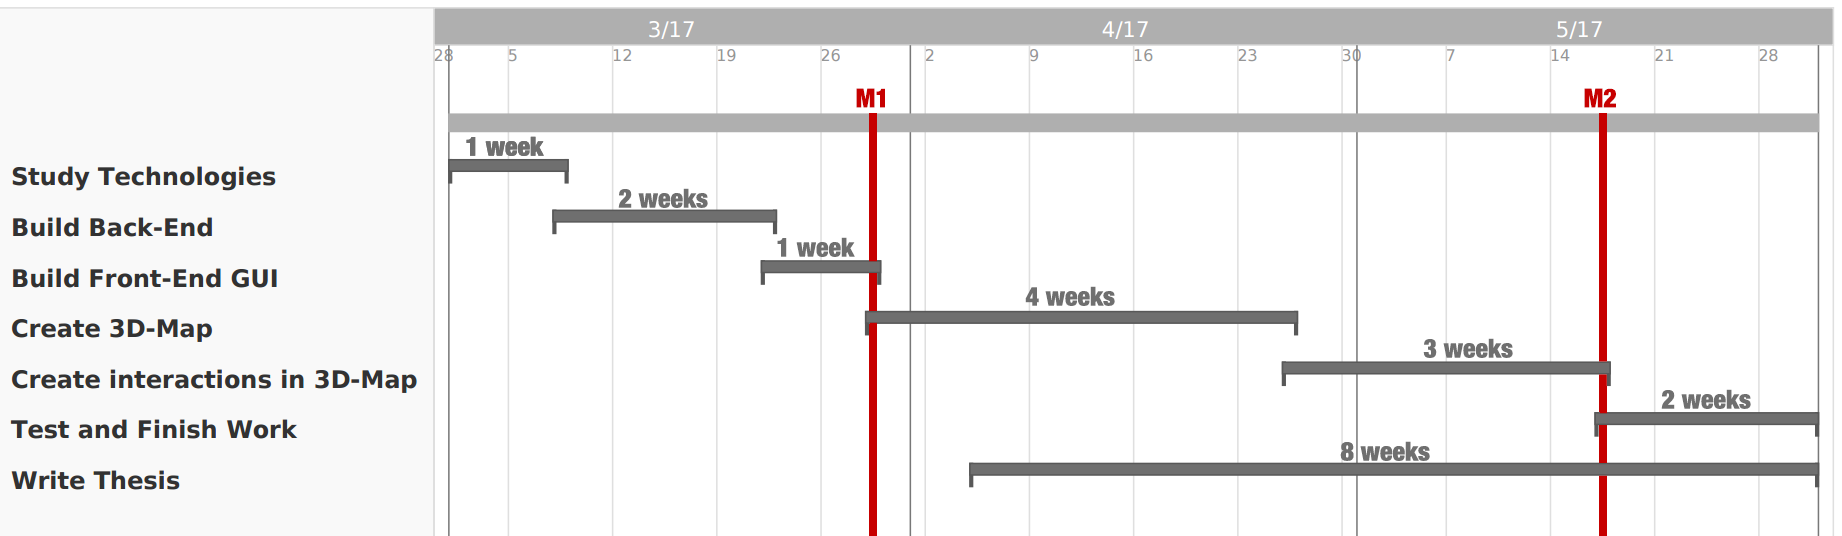
\includegraphics[scale=0.4]{Plan_timeline}

\end{document}
